% ------------ begin cheatsheet
\documentclass[a4paper]{article}
\usepackage[a4paper,margin=0.15in]{geometry}
\usepackage{multicol}

\usepackage{amsmath, amssymb}
\usepackage{enumitem}
\usepackage{graphicx}

\usepackage{ulem}
\usepackage{makecell}

% math
\newcommand{\abs}[1]{\left\lvert#1\right\rvert}

% envs
\newcommand{\ol}[1]{\begin{enumerate}#1\end{enumerate}}
\newcommand{\oll}[1]{\begin{enumerate}[leftmargin=*]#1\end{enumerate}}
\newcommand{\ul}[1]{\begin{itemize}#1\end{itemize}}
\newcommand{\ull}[1]{\begin{itemize}[leftmargin=*]#1\end{itemize}}

\graphicspath{ {./images/} }
\pagestyle{empty}
\setlength{\columnseprule}{0.3pt}

% reduce spacing before and after headers
\newcommand{\uppercaseandunderline}[1]{\uline{\uppercase{#1}}}

\makeatletter
\renewcommand{\section}{
  \@startsection{section}{1}{0pt}{1ex}{1.2ex} {\raggedleft\normalfont\normalsize\bfseries\uppercaseandunderline}}
\renewcommand{\subsection}{
  \@startsection{subsection}{2}{0pt}{1ex}{1.2ex} {\raggedleft\normalfont\small\bfseries\fbox}}
\renewcommand{\subsubsection}{
  \@startsection{subsubsection}{3}{0pt}{1ex}{0.8ex} {\raggedleft\normalfont\footnotesize\bfseries\uline}}
\renewcommand{\paragraph}{
  \@startsection{paragraph}{4}{0pt}{1.5ex}{-0.8em}{\normalfont\bfseries}}
% ------------ end cheatsheet

\newcommand{\unit}[1]{\ensuremath{\, \mathrm{#1}}}
\setlist{itemsep=0.2pt, topsep=2pt}

\begin{document}
\footnotesize
\setlength{\abovedisplayskip}{4pt}
\setlength{\belowdisplayskip}{4pt}
\setlength{\abovedisplayshortskip}{4pt}
\setlength{\belowdisplayshortskip}{4pt}
\begin{multicols*}{3}
  \part*{\centering \underline{PC1201}}
\section*{Misc}
  \paragraph{Notation}
    \ull {
      \item $\vec{F}_{ab}$: Force on $a$ due to $b$
    }
  \paragraph{Common prefixes}
    \begin{center}
      \begin{tabular}{ |ccc| }
        \hline
        \textbf{Prefix} & \textbf{Abbrev}. & \textbf{Power of 10} \\ \hline
        mega & M & $10^6$ \\ \hline
        kilo & k & $10^3$ \\ \hline
        centi & c & $10^{-2}$ \\ \hline
        milli & m & $10^{-3}$ \\ \hline
        micro & $\mu$ & $10^{-6}$ \\ \hline
        nano & n & $10^{-9}$ \\ \hline
        pico & p & $10^{-12}$ \\ \hline
      \end{tabular}
    \end{center}
  \paragraph{Units}
    \begin{center}
      \begin{tabular}{ |ccc| }
        \hline
        \textbf{Concept} & \textbf{Unit} & \textbf{Alternative} \\ \hline
        Force & N & \unit{kg \, m \, s^{-2}} \\ \hline
        Energy & J & \unit{Nm} \\ \hline
        Power & W & \unit{J \, s^{-1}} \\ \hline
        \hline
        Charge & C & - \\ \hline
        E-field & \unit{N \, C^{-1}} & \unit{V \, m^{-1}} \\ \hline
        Potential & V & \unit{J C^{-1}} \\ \hline
        Capacitance & F & \unit{C \, V^{-1}} \\ \hline
        Current & A & \unit{C \, s^{-1}} \\ \hline
        Resistance & $\Omega$ & \unit{V \, A^{-1}} \\ \hline
        \hline
        B-field & T & - \\ \hline
        Flux & Wb & \unit{T \, m^2} \\ \hline
      \end{tabular}
    \end{center}
  \subsection*{Triangles} \noindent
    Given a triangle with side lengths $a,b,c$ and angles $A,B,C$, with angle $k$ opposite to side $K$,
    \paragraph{Sine rule} $\displaystyle \frac{a}{\sin A} = \frac{b}{\sin B} = \frac{c}{\sin C}$
    \paragraph{Cosine rule} $\displaystyle c^2 = a^2 + b^2 - 2ab\cos C$
  \subsection*{Problem solving techniques}
    \ull {
      \item Write down ALL info given, and unknowns
      \item Some relevant info might be expressed only in words (e.g. starts from rest)
      \item Change to SI units
    }
\section*{Kinematics}
  \paragraph{Ticker tape} Dots are drawn every fixed interval.
    \ull {
      \item Larger gap $\Rightarrow$ faster speed
      \item Increasing gap size $\Rightarrow$ acceleration
    }
  \paragraph{SUVAT}
    \begin{align*}
      s &= ut + \frac{1}{2}at^2 & v &= u + at \\
      v^2 &= u^2 + 2as & s &= \frac{1}{2}(u+v)t
    \end{align*}
  \subsection*{Projectile Motion}
    \paragraph{Trajectory} Parabola, only depending on the initial velocity $\vec{u}$.
      \[ y = x \tan \theta - \frac{gx^2}{2u^2 \cos^2\theta} \]
      \ull {
        \item Velocity is tangent to trajectory.
        \item $v_y = 0$ at top of trajectory.
        \item $v_x$ is constant throughout trajectory.
      }
    \paragraph{Height} $H = \dfrac{u^2 \sin^2\theta}{2g}$
    \paragraph{Range} $R = \dfrac{u^2 \sin(2\theta)}{g}$
  \subsection*{Circular motion}
    \paragraph{Centripetal acceleration} keeps an object moving in a circle without changing its speed
      \[ a_c = \frac{v^2}{r} \]
      \ull {
        \item $a_c$ is always $\perp$ to $v$
        \item If speed is changing, there is a component of acceleration, $a_t$, not $\perp$ to $v$
      }
  \subsection*{Relative motion}
    \paragraph{Notation} $\vec{x}_{\text{object} \vert \text{ref frame}}$
    \paragraph{Relation} Applies also to velocity, and to 2D
      \[ \vec{x}_{A \vert B} = \vec{x}_{A \vert O} - \vec{x}_{B \vert O} = \vec{x}_{A \vert O} + \vec{x}_{O \vert B} \]
\section*{Dynamics}
  \subsection*{Forces}
    \paragraph{\uline{Gravity}} $W = mg$
    \paragraph{\uline{Tension}}
      \ull {
        \item Same throughout the whole rope
        \item Direction is along the rope
        \item Acts away from body of interest
        \item \uline{Breaking tension} is the max value of tension the rope can withstand before breaking
      }
    \paragraph{\uline{Normal}} A contact force that acts in the direction perpendicular to the surface
    \subsubsection*{Friction} \noindent
      A contact force that acts opposite to the motion, resisting
      \ull {
        \item Motion (Kinetic friction, $f_k$)
        \item Tendency to move (Static friction, $f_s$)
      }
      \paragraph{Kinetic} $f_k = \mu_k N$
      \paragraph{Static} varies from 0 to max value $f_{s_\text{max}}$, depending on the force exerted. The maximum static friction obeys
      \[ f_{s_\text{max}} = \mu_s N \]
      \ull {
        \item In general, $f_k \leq f_{s_\text{max}}$
        \item An object cannot have static and kinetic friction at the same time
      }
    \paragraph{\uline{Elastic}} Known as a restoring force, acting in the opposite direction of $\Delta \vec{x}$.
      \[ \vec{F} = -k \Delta \vec{x} \]
  \subsection*{Newton's laws}
    \paragraph{First} An object will not change its motion unless a force acts on it
    \paragraph{Second} $\vec{F} = m \vec{a}$, and vector superposition
    \paragraph{Third} Every action has an equal and opposite reaction (that acts on a different object)
      \ull{ \item Reaction pair for weight is not the normal force (both act on same object) }
  \subsection*{Two-body systems}
    \ull {
      \item Can consider each body separately
      \item Can consider both bodies together (do not include any action-reaction pairs)
    }
  \subsection*{Circular motion}
    \paragraph{Centripetal force} $F_c = ma_c = \dfrac{mv^2}{r}$
    \paragraph{Orbital motion}
      \ull {
        \item If we launch a projectile horizontally at the right speed, the curve of the falling projectile matches the curve of the earth
        \item An object in such a \uline{circular} orbit is in constant free fall, only being acted on by gravity. Hence,
          \begin{align*}
            mg &= \frac{mv^2}{r} \\
            v &= \sqrt{rg}
          \end{align*}
        \item Natural orbits tend to be more elliptical
      }
  \subsection*{Apparent weight}
    \paragraph{Normal force} Our apparent weight changes if $N \neq mg$.
      \ull {
        \item If $N < mg$, we feel lighter (lift accelerating down)
        \item If $N > mg$, we feel heavier (lift accelerating up)
        \item If $N = 0$, we are weightless (free fall)
      }
      We can experience this in elevators, vertical circular motion, orbitting satellites, etc.
  \subsection*{Problem solving techniques}
    \ull {
      \item Draw sketch of entire system
      \item Isolate SINGLE body to draw FBD, with forces acting ON the body
      \item Action-reaction pairs should NOT appear in same FBD (they act on different bodies)
      \item Choose positive axis that aligns with net $\vec{a}$
      \item Start with $\sum F = 0$ or $\sum F = ma$
      \item Do NOT assume $N = mg$
    }
\section*{Work, Energy, Power}
  \subsection*{Work}
    \ull {
      \item Is a transfer of energy, done on a system by an external agent
      \item Positive work done should increase energy of system
      \item $F$ is in same dir. as $s \Rightarrow$ +ve work done
        \[ W = F_\parallel s = Fs \cos \theta \]
        where $F_\parallel$ is component of $F$ parallel to $s$
      \item Work done is area under graph of $F-x$
    }
  \subsection*{Energy}
    \paragraph{\uline{Kinetic}} $\displaystyle W = K_f - K_i = \frac{1}{2}mv^2 - \frac{1}{2}mu^2$
    \subsubsection*{Potential}
      \ull {
        \item Stored energy due to condition of object/force of interaction between objects
        \item Only allowed by conservative forces, where work done depends only on position, and is independent of the path 
        \item When conservative forces do +ve work on the object, the potential energy of the object decreases
      }
      \paragraph{Gravitational} $\Delta U_g = mgh$
      \paragraph{Elastic} $\Delta U_s = \frac{1}{2}k(\Delta x)^2$
    \subsubsection*{Conservation of energy} \noindent
      In an isolated/closed system, total energy remains constant
      \[ \Delta E = 0 \Rightarrow \sum E_f = \sum E_i \]
      In a non-isolated/open system,
      \[ \Delta E = W \Rightarrow \sum E_f - \sum E_i = W \]
  \subsection*{Power} \noindent
    Rate of energy transfer
    \[ P = \frac{\Delta E}{t} = \frac{W}{t} \]
    Kinematics (if acceleration is 0)
    \[ P = \frac{Fs}{t} = Fv \]
\section*{Momentum} \noindent
  \[ p = mv \]
  \begin{center}
    \begin{tabular}{ |c|c|c| }
      \hline
      Collision & Elastic & Inelastic \\ \hline
      Momentum & Conserved & Conserved \\ \hline
      KE & Conserved & Not conserved \\ \hline
    \end{tabular}
  \end{center}
  \subsubsection*{Elastic collisions} \noindent
    Use equations 1 and 2, or 1 and 3 to solve. To check a collision is elastic, use 2.
    \begin{align*}
      m_1u_1 + m_2u_2 &= m_1v_1 + m_2v_2 \\
      \frac{1}{2} m_1 u_1^2 + \frac{1}{2} m_2u_2^2 &= \frac{1}{2} m_1v_1^2 + \frac{1}{2} m_2v_2^2 \\
      v_2 - v_1 &= -(u_2 - u_1)
    \end{align*}
  \subsubsection*{Impulse} \noindent
    $J$ is the area under the $F-t$ graph
    \begin{align*}
      J &= p_f - p_i = \Delta p \\
      J &= F_\text{avg} \Delta t
    \end{align*}
\section*{Electric charges}
  \subsection*{Charges}
    \paragraph{Types} +ve charges: Protons, -ve charges: Electrons
    \paragraph{Charge of an object}
      \ull {
        \item Neutral if it has equal amounts of +ve and -ve charges
        \item +vely charged if it has an excess of protons
        \item -vely charged if it has an excess of protons
        \item Protons are tightly bounded to nucleus, so they cannot be added/removed from an atom
      }
    \paragraph{Conservation of charge} One cannot create/destroy charges; one can only transfer charges from one body to another
    \paragraph{Interaction} Like charges repel, unlike charges attract
  \subsection*{Insulators}
    \paragraph{Definition} Materials that do not allow electrons to flow freely
    \paragraph{Charging} By friction, molecular bonds are broken, allowing a neutral molecule to split into positive and negative parts
  \subsection*{Conductors}
    \paragraph{Definition} Materials that allow electrons to flow freely
    \paragraph{Polarization} is a separation of charges within an object
    \subsubsection*{Charging}
      \paragraph{Charging by contact}
        \ull {
          \item Touch a conductor with an initially charged object
          \item Charges will flow to/from the conductor, leaving it with a net charge
          \item The charges will spread through the conductor rapidly
          \item The initially charged object will have less charge
        }
      \paragraph{Discharging by contact (grounding)}
        \ull {
          \item The earth can be considered as a large conductor
          \item Grounding a charged conductor is basically allowing it to make contact with earth
          \item If we ground a -vely charged object, electrons flow from object to earth
          \item If we ground a +vely charged object, electrons flow from earth to  to object
        }
      \paragraph{Charging by induction}
        \ull {
          \item Bring a charged object very near a conductor (without touching)
          \item Conductor will be polarized
          \item Ground the conductor
          \item Remove grounding wire and charged object
          \item Conductor wil now have a net charge
        }
\section*{Electric force}
  \subsection*{Coulomb's law} \noindent
    Two charges exert a force on each other
    \paragraph{Magnitude} $\displaystyle \abs{\vec{F}_{12}} = \abs{\vec{F}_{21}} = \frac{k\abs{q_1}\abs{q_2}}{r^2}$
    \paragraph{Direction}
      \ull {
        \item Along line joining two points
        \item Repulsive for like charges, attractive for unlike charges
      }
    \paragraph{Limitation}
      \ull {
        \item Only applies to point charges, but objects may be modeled as point charges if the $r$ is much larger than their size
        \item Only applies to static charges, but this module focuses on static charges
      }
\section*{Electric field} \noindent
  Explains how $q_1$ can be aware of another charge $q_0$
  \subsection*{E-field for point charge}
    \paragraph{Magnitude} We use a test charge $q_\text{test}$ to help quantify the E-field strength:
      \[ \abs{\vec{E}} = \frac{\abs{\vec{F}}}{q_\text{test}} = \frac{k\abs{q_0}}{r^2} \]
      A charge $q_1$ in an E-field due to $q_0$ experiences a force
      \[ \abs{\vec{F}} = \abs{q_1}\abs{\vec{E}} = \frac{k \abs{q_0} \abs{q_1}}{r^2} \]
    \paragraph{Direction} Defined to be the direction of the force experienced by a positive $q_\text{test}$
      \begin{center}
        \begin{tabular}{ |c|c|c| }
          \hline
          & +ve $q_\text{test}$ & -ve $q_\text{test}$ \\ \hline
          Field & Points away & Points towards \\ \hline
          Force & \makecell{Same dir.\\as field} & \makecell{Opposite dir.\\from field} \\ \hline
        \end{tabular}
      \end{center}
  \subsection*{E-field lines} \noindent
    Exist at every point in space, just a representative sample
    \paragraph{Magnitude} Higher density of field lines $\Rightarrow$ stronger field
    \paragraph{Direction}
      \ull {
        \item E-field vector is tangent to E-field line
        \item Field lines do not cross
        \item Field lines start from +ve charges and end at -ve charges
      }
  \subsection*{E-field for sphere} \noindent
    Let $R$ be the radius of the sphere. The following applies to:
    \ull {
      \item Thin insulating shell with uniform distribution
      \item Thin conducting shell (assume no charge nearby)
      \item Conducting sphere (assume no charge nearby)
    }
    \paragraph{Outside sphere} Let $Q$ be the total charge on the sphere. Let $r$ be the distance to the centre of the sphere.
      \[ \abs{\vec{E}} = \frac{k\abs{Q}}{r^2} \]
    \paragraph{Inside sphere} Inside the sphere, there is no e-field due to symmetry
  \subsection*{E-field for infinite sheet/plate}
    \ull {
      \item We can approximate most large sheets/plates as infinite sheets/plates
      \item We use this setup for parallel plate capacitors
    }
    \paragraph{Magnitude} Let $Q$ be the total charge on the plate. Let $A$ be the area of each plate.
      \[ \abs{\vec{E}} = \frac{\abs{Q}}{2 \varepsilon_0 A} \]
  \subsection*{E-field for dipole}
    \paragraph{Direction} \noindent
      \begin{center}
        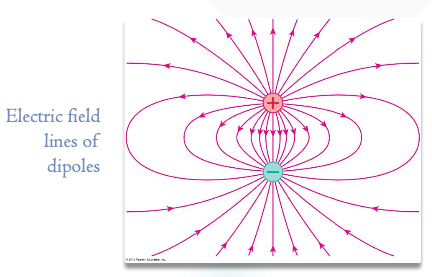
\includegraphics[width=0.25\textwidth]{dipole_field_lines}
      \end{center}
  \subsection*{E-field in conductors}
    \ull {
      \item We only consider conductors in electric equilibrium (charges not moving), so $\vec{E} = 0$
      \item Excess charges reside only on the surface, congregating at sharp points
      \item E-fields are perpendicular to surface
    }
  \subsection*{Misc}
    \paragraph{Dielectric breakdown} When E-fields within insulators get too strong, it may fail to act as an insulator, turning into a conductor, allowing charges to flow
    \paragraph{Screening in conductors} When conductors are placed in an E-field, any void in the conductor will also have $\vec{E} = 0$ (Faraday's cage / electrostatic shielding)
\section*{Electric potential\\energy}
  \subsection*{Interaction EPE for a point charge}
    \paragraph{Magnitude} A charge $q_1$ will have EPE if another charge $q_2$ is present
      \[ U_{q_1} = \frac{k q_1 q_2}{r} = U_{q_2} \]
    \paragraph{Alternative} Based on the definition of electric potential later, we also have
      \[ \Delta U = q \Delta V \]
    \paragraph{Zero point} $U \rightarrow 0$ as $r \rightarrow \infty$, i.e. when there are no charges around
    \paragraph{Sign} Similar charges have positive $U$, while opposite charges have negative $U$.
  \subsection*{Interaction EPE vs electric force} \noindent \vspace{-6mm}
    \paragraph{$\Delta U$ vs $\vec{F}_\text{ext}$}
      Work done is given by
      \[ W = \abs{\vec{F}_\text{ext}} d \cos\theta \]
      where $d$ is +ve in the direction of displacement, and $\theta$ is the angle between $\vec{F}_\text{ext}$ and $d$. We can also define work done as
      \[ W = \Delta U = U_f - U_i \]
      Hence,
      \ull {
        \item $\theta = 0 \Rightarrow$ same dir. $\Rightarrow W = \vec{F}_\text{ext} d > 0 \Rightarrow \Delta U > 0$
        \item $\theta = 180 \Rightarrow$ diff dir. $\Rightarrow W = \vec{F}_\text{ext} d < 0 \Rightarrow \Delta U < 0$
      }
      Here, $\Delta U$ is the work done on the charge to bring it from initial point $i$ to final point $f$.
    \paragraph{$\Delta U$ vs Coulomb's force $\vec{F}$}
      In order to move the charged object at constant velocity, we need $\vec{a} = 0$, so we have to oppose Coulomb's force, so
      \[ \vec{F} = -\vec{F}_\text{ext} \]
      This case has a negative sign, so
      \ull {
        \item $\vec{F}$ and $d$ same dir. $\Rightarrow \Delta U < 0$
        \item $\vec{F}$ and $d$ diff dir. $\Rightarrow \Delta U > 0$
      }
  \subsection*{Configuration EPE} \noindent
    Work required to bring the charges from infinity to build this configuration
    \[ U = \sum_{i<j} \frac{k q_i q_j}{r_{ij}} \]
\section*{Electric potential}
  \ull {
    \item Like E-field, electric potential explains how a charge can be aware of the presence of another charge
    \item But E-field is about force per charge while electric potential is about work done/energy per charge
  }
  \subsection*{Electric potential for point charge}
    \paragraph{Magnitude} Similar to E-field, we obtain magnitude by placing a test charge $q_\text{test}$ at the point we are interested in.
      \[ V = \frac{U}{q_\text{test}} = \frac{k q_0}{r} \]
      where $q_0$ is the charge that created the electric potential. Thus, a charge $q_1$ in a potential due to $q_0$ has energy
      \[ U = q_1 V = \frac{k q_0 q_1}{r} \]
  \subsection*{Electric potential for sphere/shell} \noindent
    Let $R$ be the radius of the sphere. The following applies to:
    \ull {
      \item Thin insulating shell with uniform distribution
      \item Thin conducting shell (assume no charge nearby)
      \item Conducting sphere (assume no charge nearby)
    }
    \paragraph{Outside sphere} Let $Q$ be the total charge on the sphere. Let $r$ be the distance to the centre of the sphere.
      \[ V = \frac{kQ}{r} \]
    \paragraph{Inside sphere} Inside the sphere, potential is constant.
      \[ V = \frac{kQ}{R} \]
  \subsection*{Equipotential surfaces}
    \ull {
      \item Lines/surfaces of the same potential, so moving a charge along the line does not change EPE
      \item PD between each adjacent pair of equipotential lines is the same
    }
  \subsection*{Relationship to $\vec{E}$}
    \ull {
      \item E-field points in direction of decreasing potential
        \ull {
          \item PD establishes E-field
          \item A charge in a PD experiences a force
        }
      \item E-fields are perpendicular to equipotential lines
      \item If E-field is constant, then
        \[ \abs{\vec{E}} = \frac{\abs{\Delta V}}{d} \]
        where $d$ is the distance between the two points (parallel to $\vec{E}$), and $\Delta V$ is the PD between the two points.
      \begin{center}
        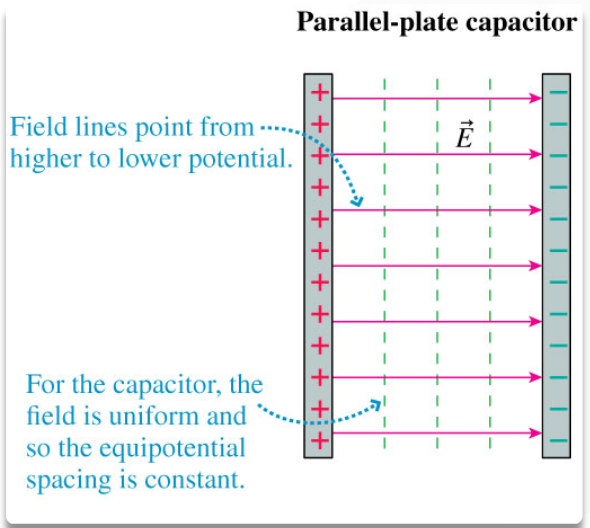
\includegraphics[width=0.25\textwidth]{potential_and_e_field}
      \end{center}
    }
  \subsection*{Moving charge in a field}
    \oll {
      \item Charge $q$ moving from A to B in a PD $\Delta V$
        \[ \Delta U = q \Delta V \]
      \item Charge $q$ moving from A to B in a constant $\vec{E}$ field
        \[ \Delta \vec{V} = \abs{\vec{E}} d \]
    }
  \subsection*{L12 QC6} 
    \ull {
      \item Charges move because of a PD, so they stop moving once there is no PD
      \item If two conductors are connected via a wire, charges redistribute equally only if the two conductors are identical.
    }
\section*{Capacitance, current,\\resistance}
  \subsection*{Capacitor}
    \paragraph{Capacitance} A capacitor stores electric charges, and consists of two equally and oppositely charged parts that are some distance apart. The capacitance $C$ is given as:
      \[ C = \frac{Q}{\Delta V} = \frac{Q}{Ed} = \kappa \frac{\varepsilon_0 A}{d} \]
      \ull {
        \item $Q$ is the amount of charge the capacitor can hold, given PD between the plates $\Delta V$
        \item $\kappa$ is the dielectric constant, 1 in air, others will be given
        \item RHS is always true, even if the capacitor is disconnected
      }
    \paragraph{Electric field} Proved in assignment 2:
      \[ \abs{\vec{E}} = \frac{Q}{\varepsilon_0 A} \]
    \paragraph{Dielectric in a capacitor}
      \ull {
        \item As mentioned above, it introduces $\kappa$ into the equation
        \item (CA2 Q10) If there are multiple dielectrics, then treat them as capacitors, and handle series/parallel correctly
      }
    \paragraph{Energy} Energy stored in a capacitor is equal to the work done to charge it
        \[ U = \frac{1}{2} Q \Delta V = \frac{Q^2}{2C} = \frac{1}{2} C (\Delta V)^2 \]
    \paragraph{Energy density} The capacitor's energy is stored in the electric field between the plates.
      \[ U = \frac{1}{2} C (\Delta V)^2 = \frac{1}{2} \frac{\varepsilon_0 A}{d} (Ed)^2 = \frac{1}{2} \varepsilon_0 E^2 (Ad) \]
      In order to be independent of the dimensions of the capacitor, define $u = \dfrac{U}{Ad}$ to be the energy density, so we have
      \[ u = \frac{C (\Delta V)^2}{2Ad} = \frac{1}{2} \varepsilon_0 E^2 \]
  \subsection*{Current}
    \ull {
      \item Rate of flow of charge $I = \dfrac{Q}{\Delta t}$
      \item Defined to be the direction of flow of positive charges (although electrons are the ones flowing)
      \item $\Delta V$ exists $\Rightarrow \vec{E}$ exists $\Rightarrow$ force exists $\Rightarrow$ electrons move (in opposite direction of $\vec{E}$)
    }
    \paragraph{EMF source, $\varepsilon$} (Creates and) maintains a constant PD by moving +ve charges against the electric field, opposing Coulomb's force
    \paragraph{Power supplied by EMF source} The +ve charges gain potential energy $U = q \Delta V$, so a battery supplies energy $U = q \varepsilon$.
      \[ P = \frac{U}{\Delta t} = \frac{q \Delta V}{\Delta t} = I \Delta V = I \varepsilon \]
  \subsection*{Resistance}
    \ull {
      \item For ohmic materials, which have constant resistance, Ohm's law holds true: $R = \dfrac{\Delta V}{I}$
      \item Can assume the materials are ohmic unless otherwise stated
    }
    \paragraph{Computing resistance for a material}
      \[ R = \frac{\rho l}{A} \]
      where $\rho$ is the resistivity (given), $l$ is the length of the conductor, $A$ is the cross sectional area.
    \paragraph{Power} For ohmic resistors,
      \[ P = I \Delta V = I^2 R = \frac{(\Delta V)^2}{R} \]
      \ull {
        \item Power ratings in household appliances are based off a constant voltage (230V in Singapore), so they indirectly give us the resistance of the appliance
        \item Lower power rating $\Rightarrow$ higher resistance
        \item Kilowatt hour (kWh) is the \uline{energy} that a 1kW power source uses up in 1 hour
      }
\section*{DC circuits}
  \paragraph{Battery} Positive terminal is the longer line
    \subsection*{Resistors}
      \begin{center}
        \begin{tabular}{ |c|c|c| }
          \hline
          & Series & Parallel \\ \hline
          PD & Sum & Same \\ \hline
          Current & Same & Sum \\ \hline
          Resistance & Sum & \makecell{Reciprocal of \\ (sum of \\ reciprocals)} \\ \hline
        \end{tabular}
      \end{center}
    \subsection*{Capacitor}
      \begin{center}
        \begin{tabular}{ |c|c|c| }
          \hline
          & Series & Parallel \\ \hline
          PD & Sum & Same \\ \hline
          Charge & Same & Sum \\ \hline
          Capacitance & \makecell{Reciprocal of \\ (sum of \\ reciprocals)} & Sum \\ \hline
        \end{tabular}
      \end{center}
    \subsection*{Kirchhoff}
      \paragraph{Parallel vs series}
        \ull {
          \item Two elements are in parallel if any loop contains only those two elements
          \item Two elements are in series if every loop contains only both those elements
        }
      \paragraph{Junction rule} $\displaystyle \sum I_\text{in} = \sum I_\text{out}$
      \paragraph{Loop rule} sum of PD along loop is 0
      \paragraph{How $V$ changes across circuit elements}
        \ull {
          \item Battery: Positive plate has higher potential than negative plate
          \item Resistor: Potential decreases in the direction of current (depends on the emf or the setup)
          \item If travel direction is towards lower potential, then $\Delta V$ is negative, vice versa
        }
        \begin{center}
          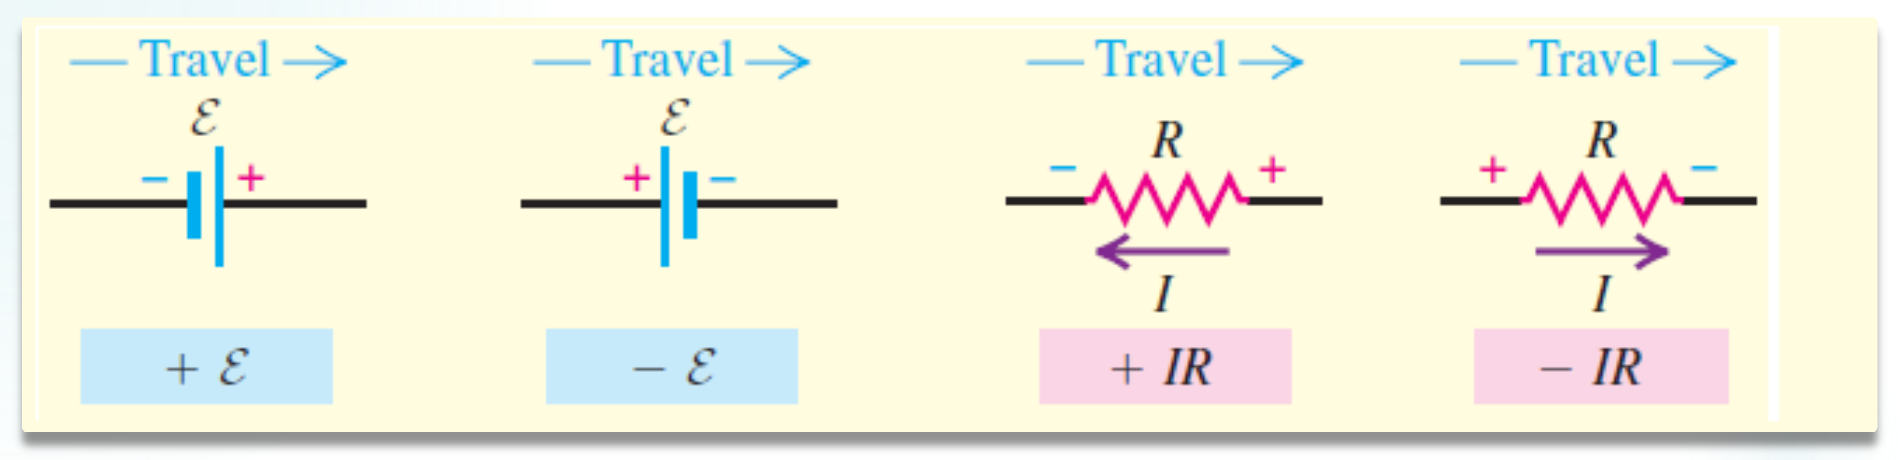
\includegraphics[width=0.3\textwidth]{how_v_changes}
        \end{center}
      \paragraph{Strategy}
        \ull {
          \item Label everything and write down all info
          \item Fix direction of currents
          \item Apply loop rule $n-1$ times, by going in a loop and comparing with current direction
          \item Apply junction rule using current direction
        }
\section*{Magnetic field}
  \paragraph{Magnet} Has ``inherent magnetic moments'' that are aligned, so dropping/heating will harm the magnet
  \paragraph{Earth is a magnet}
    \ull {
      \item The magnetic north pole is (near) the geographic south pole of the earth
      \item A compass needle points N because the N pole of the compass needle is attracted to the magnetic S pole of the earth, which is (near) the geographic N pole of the earth
    }
  \paragraph{Magnetic field lines}
    \ull {
      \item Starts from north pole, ends at south pole
      \item Denser where field is stronger (near magnet)
      \item Never crosses
    }
  \paragraph{3D convention}
    \ull {
      \item Cross means current into page, dot means current out of page
      \item Vertical plane (up/down, west/east): used in question paper
      \item Horizontal plane (north/south, west/east): surface of the earth
      \item Other plane (up/down, north/south): visualize earth's B-field away from the equator
    }
    \begin{center}
      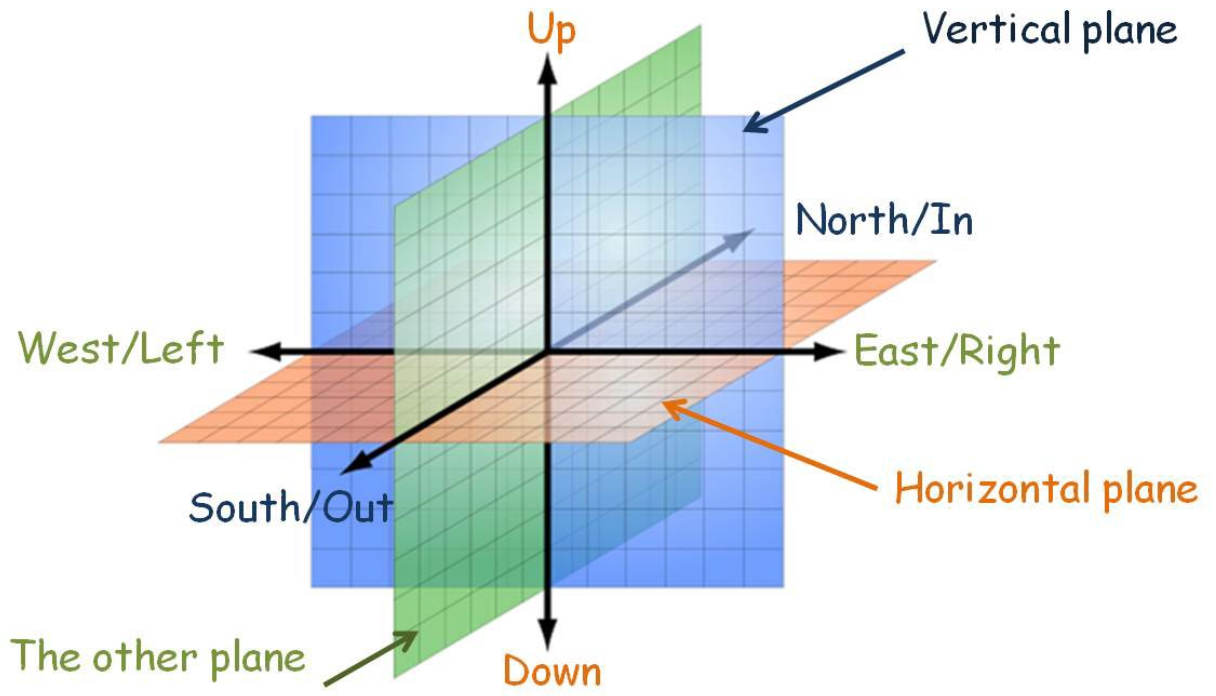
\includegraphics[width=0.3\textwidth]{planes}
    \end{center}
  \paragraph{Dip angle}
    \ull {
      \item Magnetic field at the equator is approximately horizontal
      \item Magnetic field at the poles is nearly vertical
      \item Measured with respect to the surface of the earth
    }
  \subsection*{Sources of magnetic fields}
    \paragraph{Right hand grip rule (RHGR)}
      \oll {
        \item Point your right thumb in the direction of current
        \item Wrap your fingers around the wire to indicate a circle
        \item Your fingers curl in the direction of the B-field lines around the wire
      }
    \paragraph{Moving charge (in a wire)}
      \ull {
        \item Stationary charge produces E-field, while moving charge produces B-field
        \item Magnitude is
          \[ \abs{\vec{B}} = \frac{\mu_0 I}{2 \pi r} \]
        \item Direction determined by RHGR
      }
    \paragraph{Current loop}
      \ull {
        \item Magnitude at the centre is:
          \[ \abs{\vec{B}} = \frac{\mu_0 N I}{2R} \]
          where $N$ is the number of loops
        \item Direction determined by RHGR, or
        \item Fingers curl in the current direction (along loop), thumb points in direction of B (magnetic north)
      }
    \paragraph{Solenoid}
      \ull {
        \item Magnitude inside solenoid is almost uniform
          \[ \abs{\vec{B}} = \frac{\mu_0 N I}{L} = \mu_0 n I = \frac{\mu_0 I}{2r} \]
          where $N$ is the number of turns, $n = N/L$ is the number of turns per unit length, $r$ is the radius of the cross-section of the wire
        \item Outside a solenoid is very small
          % TODO test 2 claims it is 0
        \item Magnitude outside solenoid is very small
        \item Direction: use RHGR like in current loop
        \item From Tut 6, $N = L / (2r)$. This $r$ is the radius of the cross-section of the wire, NOT the radius of the solenoid.
      }
      \begin{center}
        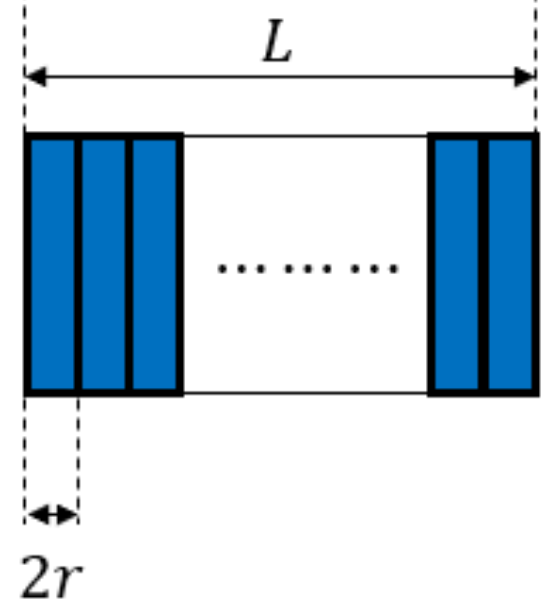
\includegraphics[width=0.12\textwidth]{solenoid_N}
      \end{center}
\section*{Magnetic force}
  \paragraph{Right hand cross rule (RHCR)}
    \oll {
      \item Point 4 fingers in the direction of $v$
      \item Rotate hand so that palm faces direction of $B$
      \item Direction of thumb is direction of the force $F$
      \item If charge is negative, flip the direction of the force
    }
  \subsection*{Force on moving charge} \noindent
    A magnetic force is exerted on a moving charge in a magnetic field
    \paragraph{Magnitude} $\abs{\vec{F}} = \abs{q} v_\perp B = \abs{q} v B \sin \alpha$
    \paragraph{Direction} use RHCR
    \paragraph{Trajectory}
    \ull {
      \item If initial $v$ is perpendicular to $B$, since $F$ is always perpendicular to $v$, we have circular motion
        \[ F = qvB = \frac{mv^2}{r} \quad\text{or}\quad r = \frac{mv}{qB} \]
      \item Otherwise, there is circular motion in the horizontal plane, but also vertical motion in the vertical axis, due to the non-zero component of $v$ parallel to the B-field. This is called helical motion.
    }
  \subsection*{Force on current-carrying wire}
    \paragraph{Magnitude} A wire has $Nq$ charge flowing in it, so we have
      \[ F = Nq vB \sin \alpha \] 
      If we multiply by $t/t$, we have
      \[ F = \frac{Nq}{t} (vt) B \sin \alpha = IlB \sin \alpha \]
      where $vt = l$ is the length of the wire, and $I = \dfrac{Nq}{t}$ is the current.
      \begin{center}
        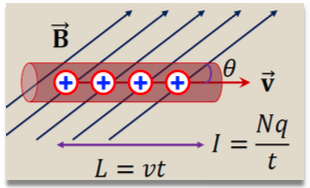
\includegraphics[width=0.15\textwidth]{current_carrying_wire}
      \end{center}
    \paragraph{Direction} use RHCR, replacing $v$ with $I$ (they are in the same direction actually)
  \subsection*{\parbox{120pt}{Force between (parallel)\\current-carrying wires}}
    \paragraph{Magnitude} Each wire exerts a force on the other, and it is symmetric:
      \[ F = F_{12} = F_{21} = I_2 l B = I_2 l \left(\frac{\mu_0 I_1}{2 \pi r}\right) \]
      where $r$ is the distance between the wires. Alternatively,
      \[ F = \frac{\mu_0 I_1 I_2 l}{2 \pi r} \]
    \paragraph{Direction} If their currents are flowing in the same direction, then the wires will attract. Otherwise they repel.
    \paragraph{Note} The B field generated by a wire does not affect itself.
  \subsection*{Cross fields} \noindent
    If we want to filter charges, we can pass them through a cross field that has both electric and magnetic forces.
    \paragraph{Direction}
      \ull {
        \item Arrange in such a way that the forces are equal and opposite (for a particular type of charge, e.g. positive), then for the negative charge it will be equal but in the same direction
        \item Thus positive charges will move straight
      }
    \paragraph{Magnitude} We have $qvB = qE$, i.e. $v = \dfrac{E}{B}$
  \subsection*{Mass spectrometer} \noindent
    A mass spectrometer is a device used to measure the mass of an atom. It uses crossed fields for a velocity selector, and the circular trajectory of a charged particle in a magnetic field, to measure the mass of an atom.
    \[ qvB = \frac{mv^2}{r} \Rightarrow m = \frac{qBr}{v} \]
    \begin{center}
      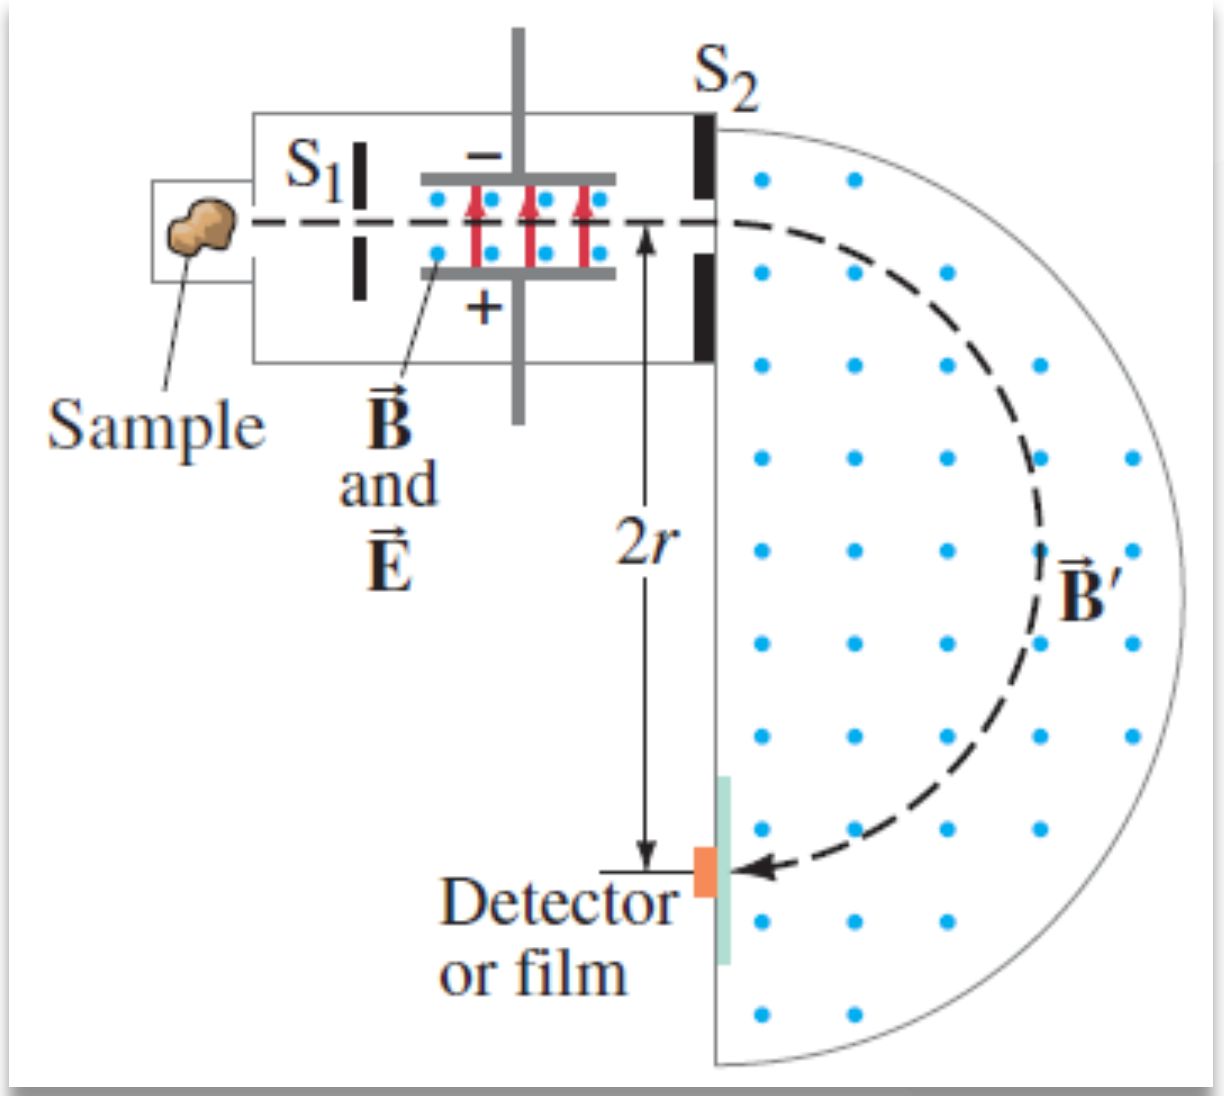
\includegraphics[width=0.2\textwidth]{mass_spectrometer}
    \end{center}
  \subsection*{Electromagnetic flowmeter} \noindent
    An electromagnetic flowmeter can measure speed of blood flow. In the presence of a B-field, positive and negative charges will separate, creating an E-field. When $F_E = F_B$, then ions travel through undeflected, and we can calculate
    \[ v = \frac{E}{B} \]
    \begin{center}
      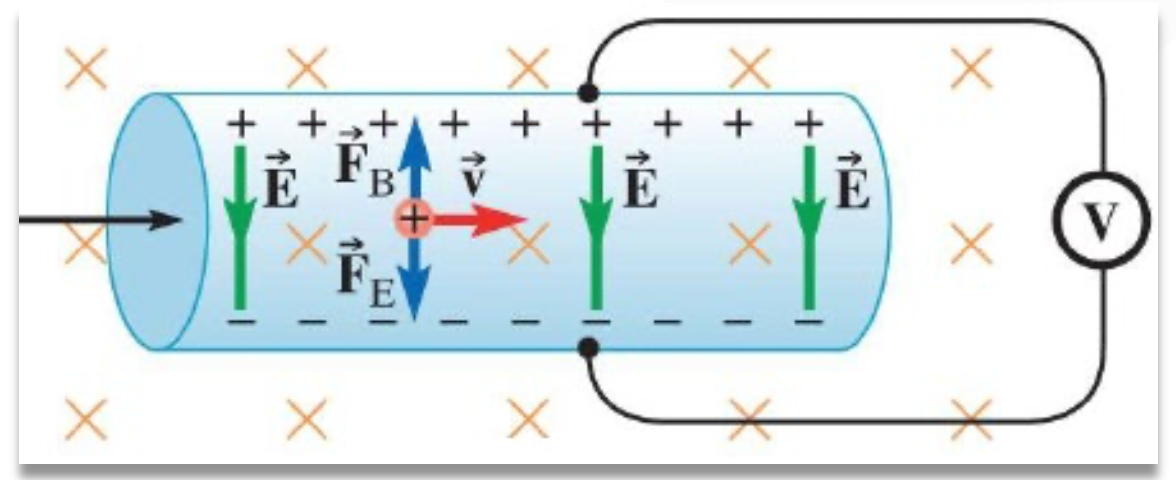
\includegraphics[width=0.2\textwidth]{electromagnetic_flowmeter}
    \end{center}
\section*{Induction}
  \subsection*{Motional EMF}
    \paragraph{How it works}
      \ull {
        \item Similar to electromagnetic flowmeter
        \item When a conductor moves perpendicular to a B-field (via $F_\text{ext}$), then $F_B$ is exerted on the charges. But $F_B$ acts in opposite directions for positive and negative charges, so there is a charge separation, leading to an EMF.
        \item The building of the EMF creates a PD, resulting in a $F_E$ that will resist $F_B$. So charges continue accumulating until $F_B = F_E$.
          \begin{align*}
            qvB &= qE \\
            vB &= \frac{\Delta V}{d} \\
            \Delta V &= Bdv
          \end{align*}
          and we rename $\varepsilon = \Delta V$ and $l = d$ to get the more well-known
          \[ \varepsilon = Blv \]
      }
    \paragraph{Induced current} If the moving conductor is connected to a circuit, then a current is induced.
      \[ I = \frac{\varepsilon}{R} = \frac{Blv}{R} \]
    \paragraph{Induced force} With the induced current, and since the conductor is moving in a B-field, we have a magnetic force
      \[ F_B = IlB = \frac{B^2 l^2 v}{R} \]
      and direction can be obtained via RHCR (with current). Note that $v$ is in the direction of $F_\text{ext}$.
  \subsection*{Magnetic flux} \noindent
    \ull {
      \item Amount of B-field that passes through a loop
      \item Magnitude is
        \[ \phi = NBA \cos \theta \]
        where $N$ is the number of loops, $A$ is the area of the loop, and $\theta$ is the angle between the axis of the loop to the B-field
      \item Axis of the loop is the line passing through the centre of the loop, so $A \cos \theta$ is like the effective area of the loop
    }
    \begin{center}
      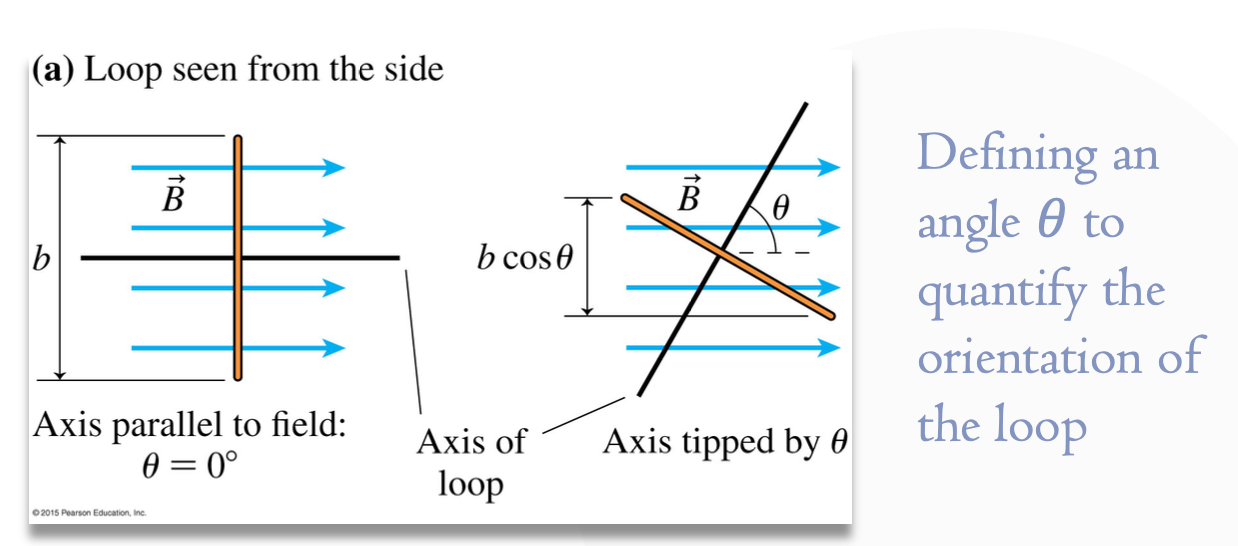
\includegraphics[width=0.25\textwidth]{flux_angle}
    \end{center}
  \subsection*{Faraday's law} \noindent
    An EMF is induced in a conducting loop if the magnetic flux through the loop changes
    \[ \varepsilon = \abs{\frac{\Delta \phi}{\Delta t}} \]
    and any of $B, A, \theta$ may cause a change in flux.
  \subsection*{Lenz's law} \noindent
    Direction of induced current is such that the induced B-field opposes the change in flux.
    \begin{equation*}
      \resizebox{\hsize}{!}{$
        \Delta \phi \rightarrow \varepsilon_\text{induced} \rightarrow I_\text{induced} \rightarrow B_\text{induced} \rightarrow \phi_\text{induced}
      $}
    \end{equation*}
    \paragraph{How to apply}
      \oll {
        \item Determine direction of B-field
        \item Determine if flux is increasing/decreasing
        \item Lenz's law states that induced B-field will oppose this change
        \item RHGR determines the direction of $I$ that induces this B-field
      }
      \begin{center}
        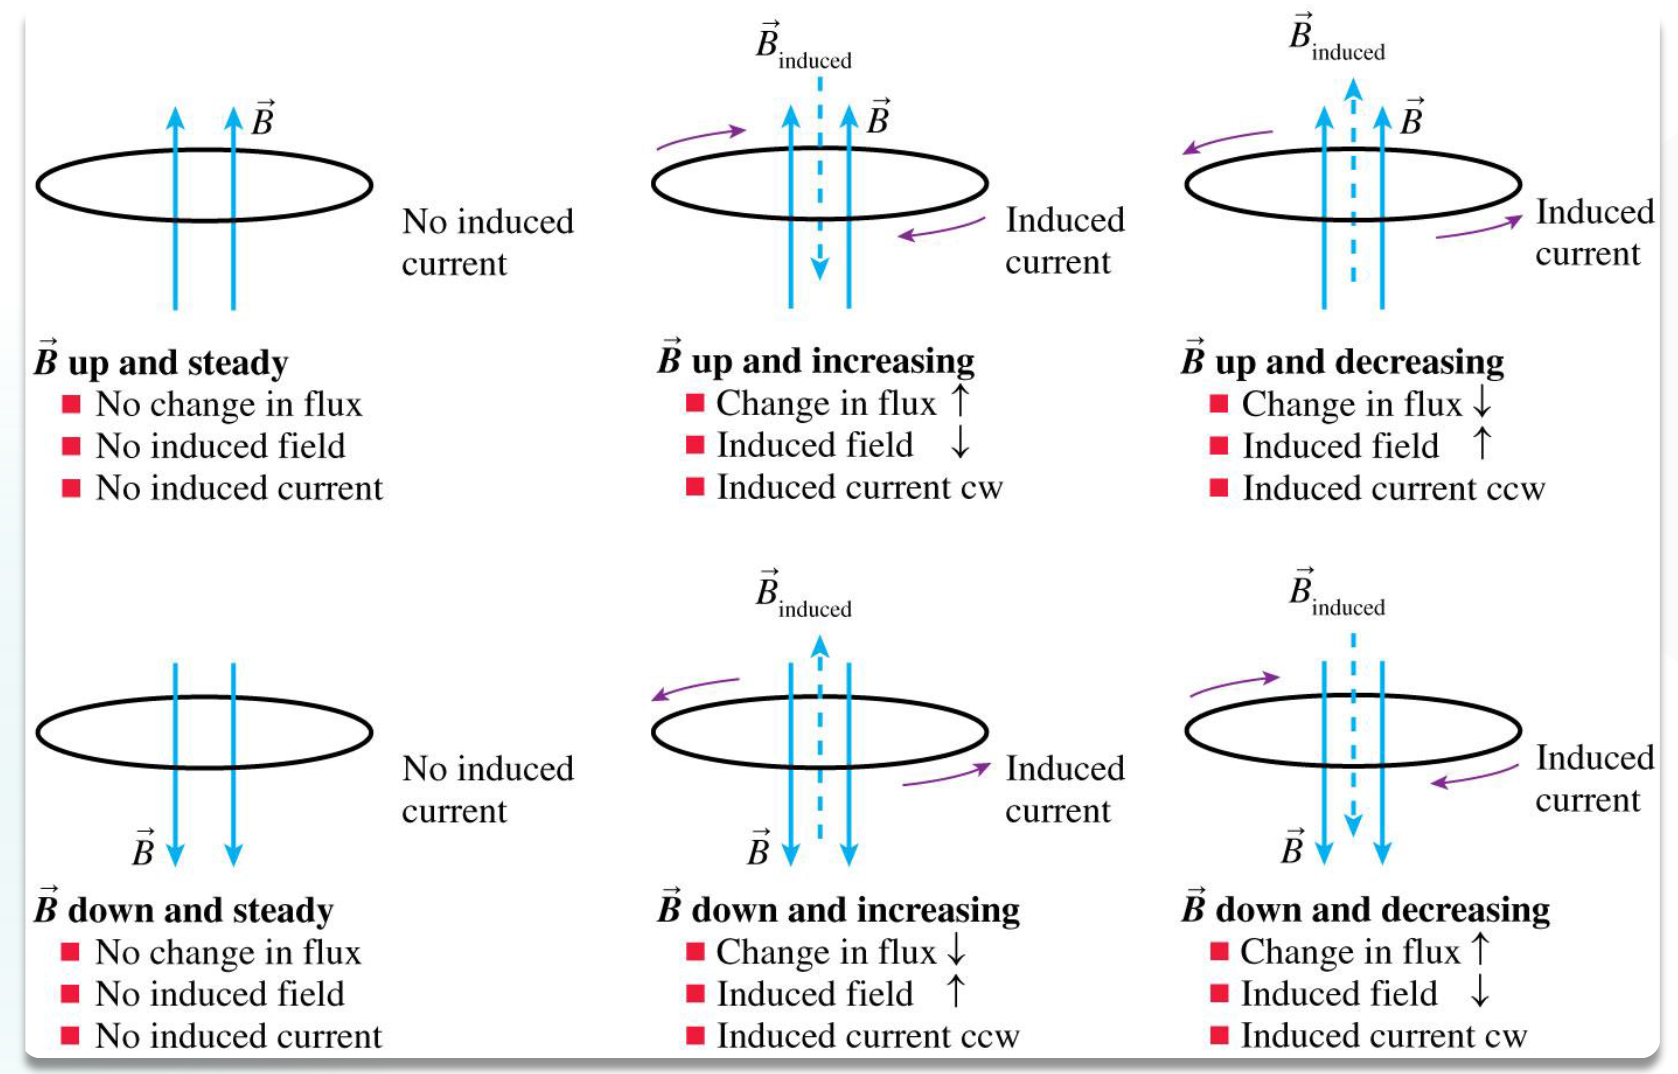
\includegraphics[width=0.25\textwidth]{lenz_law}
      \end{center}
\end{multicols*}
\end{document}
